\subsection{Attribution and Jacobian Diagnostics}
\label{sec:detail_attribution_details}
\begin{figure*}[t]
\centering
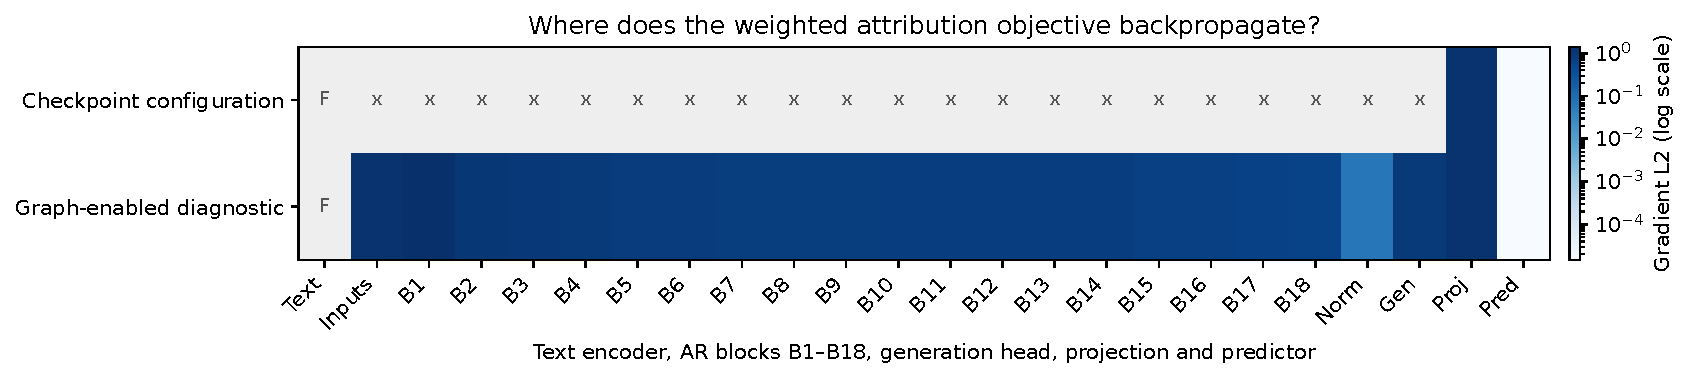
\includegraphics[width=\textwidth]{figures/attribution_gradient_reachability.pdf}
\caption{The detached attribution objective reaches auxiliary heads but not the generator. Colors show gradient $\ell_2$ norms on a logarithmic scale; ``F'' denotes a frozen module and ``x'' a disconnected path. The second row enables the attribution graph only for a same-batch connectivity test, not a newly trained model.}
\label{fig:gradient_reachability}
\end{figure*}
We test the theoretical interpretation at three levels: association between
attribution and hidden-state changes, gradient reachability of the auxiliary
objective, and direct estimates of the text-to-hidden-state Jacobian.

\paragraph{Sampling and representations.}
The 300 source-motion groups in Section~\ref{sec:latent_diagnostics} exclude
training groups and treat original/mirrored motions as one source. Selection
uses seed 123 with a test-specific offset, excluding captions that require
CLIP truncation and motions that require submotion or resampling repairs.
The frozen VQ-VAE encodes deterministic multiple-of-four center crops.
Both text conditions use identical target prefixes. Attribution averages
log-likelihood over at most 16 valid motion tokens per sample, excluding end
and padding tokens. We extract outputs from 18 Transformer blocks and final
normalization.

The 100-group intervention subset requires at least three alphabetic,
non-stopword content words, each occupying one CLIP token. One word is
perturbed at a time, with norm 0.1 or 0.25 times the median eligible-word
embedding norm, three paired Gaussian directions, and both signs.
The relative response divides the Frobenius norm of the hidden-state change
by the unperturbed-state norm. Input strengths, random-word identities, and
directions are shared across models; high/low choices follow each model's
attribution ranking.

\paragraph{Attribution--state association.}
A deterministic single-word rule supplies 235 additional altering pairs:
78 action, 79 body-part, and 78 direction edits. These pairs have no edited
motion ground truth. Attribution comparison excludes special/padding tokens,
normalizes the remaining scores, aligns identical words by occurrence, and
merges unmatched words into a residual bucket. This lexical alignment differs
from the learned pooling head's normalization over all 77 CLIP positions.
We measure Jensen--Shannon divergence (JSD) between the aligned attribution
distributions and its association with hidden-state displacement.

\begin{figure*}[t]
\centering
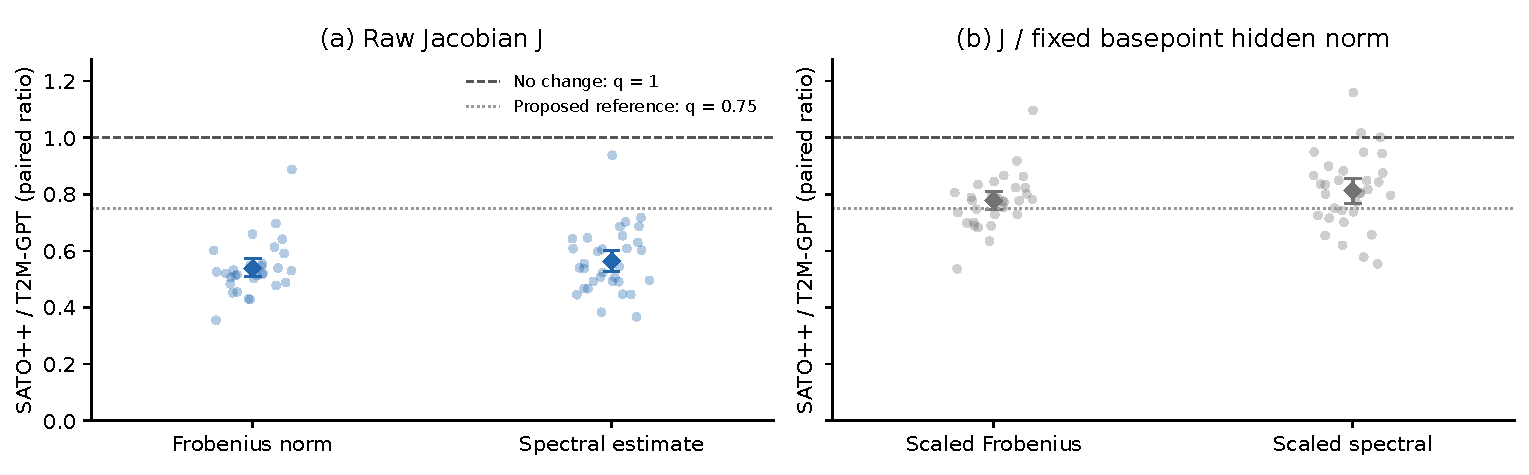
\includegraphics[width=\textwidth]{figures/jacobian_norm_ratios.pdf}
\caption{Lower average local sensitivity for COMPASS on 32 shared groups. (a) Paired ratios of raw Jacobian Frobenius norms and spectral estimates. (b) Ratios after dividing each Jacobian by its model's fixed basepoint hidden norm. Dots denote groups, diamonds means, and bars 95\% source-group bootstrap intervals. The 0.75 line is a reference hypothesis.}
\label{fig:jacobian_norms}
\end{figure*}
Figure~\ref{fig:attribution_association} reports partial Spearman correlations
controlling for frozen CLIP distance, token-count difference, lexical edit
fraction, original token count, valid prefix length, and uniform-attribution
JSD. Final-state correlations for altering pairs are 0.106 for the parent and
0.181 for COMPASS; preserving-pair values are 0.069 and 0.051. For COMPASS,
95\% source-group bootstrap intervals from 1,000 resamples are
$[0.032,0.301]$ and $[-0.021,0.128]$, respectively. The altering-pair
between-model difference is 0.075 with interval $[-0.055,0.192]$.
Thus the numerical increase does not establish a reliable association gain.

Distances between learned pooled representations correlate with final-state
distances at 0.455 (preserving) and 0.470 (altering), compared with 0.548
and 0.668 for uniform contextual-feature pooling. Mean altering displacement
also decreases from 0.399 to 0.292. These findings distinguish lower overall
sensitivity from selective compliance with a requested edit.

\paragraph{Gradient reachability.}
A fixed training batch containing two preserving and one altering pair tests
each loss under frozen CLIP and detached attribution. Generation and teacher
losses connect to 295 of 296 generator parameter tensors; the remaining
tensor is unused in the forward pass. The alignment objective
updates auxiliary pooling/predictor heads without reaching the generator.
Difference and locality losses have no gradient function.
An additional nominal 300-group validation probe overlaps the training list
and is excluded from held-out evidence.

% TODO(audit): the 1.203 / 1.48e-5 head norms come from a run whose weighted
% sum still included the variance and covariance terms. Rerun
% tools/audit_sato_gradient_connectivity.py with lambda_var=lambda_cov=0 to
% refresh these two values. The connectivity claims are unaffected.
Figure~\ref{fig:gradient_reachability} isolates the weighted sum of the
auxiliary attribution objectives.
All generator blocks and the generation head are disconnected. Projection
and predictor gradient norms are 1.203 and $1.48\times10^{-5}$.
Enabling the attribution graph on the same batch restores a generator gradient
with aggregate norm 3.809, but does not retrain the checkpoint.
For the detached configuration, the generator-only gradient cosine is
undefined and an attribution-only virtual SGD step leaves the generator
unchanged. This establishes a connectivity limitation, not a measured
risk decrease under the graph-enabled variant.

\paragraph{Direct Jacobian estimates.}
We sample 32 of the 100 intervention groups uniformly without replacement,
independently of outcomes. Let $J=\partial G_K/\partial H_{\mathrm{vis}}$,
where $G_K$ concatenates final normalized generator states over the valid
prefix and $H_{\mathrm{vis}}$ contains visible pre-contextual CLIP embeddings.
Beginning/end/padding embeddings and target prefixes are fixed.
We estimate $\|J\|_F^2$ with 32 Rademacher Hutchinson probes and $\|J\|_2$
with power iteration using Jacobian--vector and vector--Jacobian products
(JVPs/VJPs), two random starts, and at most 20 iterations. Both models meet
relative singular-value change below $10^{-3}$ and normalized
$J^\top J$ residual below 0.02 for all groups. Central differences at 0.001
and 0.01 times the sentence-median embedding norm validate the JVPs; median
relative error at the larger step is below $4\times10^{-4}$ for both models.

Mean COMPASS/parent ratios are 0.539 for the Frobenius norm and 0.563 for
the spectral estimate, with both raw ratios below one for all sampled groups
(Figure~\ref{fig:jacobian_norms}). The mean squared-Frobenius ratio is 0.298.
After division by the fixed basepoint norm $\|G_K(x)\|_F$, Frobenius and
spectral ratios are 0.776 and 0.812; the latter is below one for 29 of 32
groups. This scaling corresponds to relative response, not differentiation
of a normalized output function. Using identical baseline-ranked
high/low/random positions and three shared unit directions gives mean scaled
JVP ratios of 0.753, 0.772, and 0.781. Directions are averaged within each
group before 2,000 group-bootstrap resamples.

These measurements support lower average local sensitivity on sampled inputs,
not a uniform 0.75 contraction factor. In particular, the normalized spectral
ratio 0.812 differs from the approximate 0.75 finite-response ratio. Neither
summary verifies the directional ordering in~\eqref{eq:theory_contraction}
or the representation bridge in~\eqref{eq:theory_bridge}. Extending a local
bound to finite prompt changes would also require control along the
interpolating path, not only at its endpoints.